%! TEX root = 1_prinsipstruktur.tex
% the main TeX file which is intended to compile, :VimtexReload after adjustment
   % this file should be included in the main file
% :h vimtex-tex-root
\documentclass[../modul_skb.tex]{subfiles}
%ensure the class of docs

\begin{document}

\section{prinsip-prinsip sistem struktur dengan parameter struktur }%
\label{sec:prinsip-prinsip sistem struktur dengan parameter struktur }

\subsection{Prinsip Dasar Struktur}%
\label{sub:Prinsip Dasar Struktur}

\subsubsection{Kekuatan}%
\label{ssub:Kekuatan}

Kekuatan merupakan kemampuan elemen dan komponen struktur bangunan yang bekerja secara vertikal ataupun horizontal bangunan dalam menahan beban-beban yang timbul. Komponen struktur verikal berupa kolom berfungsi menahan gaya-gaya vertikal yang dialirkan dan disebarkan menuju sub-struktur dan pondasi bangunan. Komponen struktur horizontal berupa struktur lantai dan balok sebagai penahan beban mati dan beban hidup yang diteruskan ke kolom. (Zuhri, 2011)

\subsubsection{Kestabilan}%
\label{ssub:Kestabilan}

Kestabilan bangunan merupakan kemampuan bangunan dalam mengatasi gaya-gaya lateral dari luar, seperti angin, gempa, ataupun gaya gravitasi bumi. Hal ini dapat tercapai dari pembentuk struktur bangunan yang memberikan perilaku struktur yang stabil. (Zuhri, 2011)

\subsubsection{Keseimbangan}%
\label{ssub:Keseimbangan}

Keseimbangan merupakan perilaku massa dalam mengatasi gaya gravitasi bumi dan angin, dimana perilaku struktur dicapai dengan memberikan bidang-bidang vertikal massif yang berfungsi untuk meneruskan beban dan membentuk sudut dengan permukaan tanah. (Zuhri, 2011)

\subsection{Beban Struktur}%
\label{sub:Beban Struktur}

Pada suatu struktur bangunan, terdapat beberapa jenis beban yang bekerja. Beban-beban yang bekerja pada struktur suatu bangunan, yang diperhitungkan dalam penulisan tugas akhir ini sesuai SNI 1727-1989 adalah sebagai berikut :

\subsubsection{Beban Mati}%
\label{ssub:Beban Mati}

Ialah berat dari semua bagian dari suatu gedung yang bersifat tetap, termasuk segala unsur tambahan, penyelesaian-penyelesaian, mesinmesin. Serta peralatan tetap yang merupakan bagian tak terpisahkan dari gedung itu.

\subsubsection{Beban Hidup}%
\label{ssub:Beban Hidup}

Ialah semua beban yang terjadi akibat penghunian atau penggunaan suatu gedung, dan ke dalamnya termasuk beban-beban lantai yang berasal dari barang-barang yang dapat berpindah, mesin-mesin serta peralatan yang tidak merupakan bagian tak terpisahkan dari gedung dan dapat diganti selama masa hidup dari gedung itu, sehingga mengakibatkan perubahan dalam pembebanan lantai dan atap tersebut.

\subsubsection{Beban Gempa}%
\label{ssub:Beban Gempa}

Ialah semua beban statik ekivalen yang bekerja pada gedung atau bagian gedung yang menirukan pengaruh dan gerakan tanah akibat gempa itu. Dalam hal pengaruh gempa pada struktur gedung ditentukan berdasarkan suatu analisa dinamik maka yang diartikan dengan beban gempa di sini adalah gaya-gaya di dalam struktur tersebut yang terjadi oleh gerakan tanah akibat gempa itu.

\section{Sistem Struktur}%
\label{sec:Sistem Struktur}

\subsection{Struktur Rangka}%
\label{sub:Struktur Rangka}
Struktur Rangka adalah struktur yang terdiri dari batang-batang yang panjangnya jauh lebih besar dibandingkan dengan ukuran penampangnya Bentuk kontruksi rangka adalah perwujudan dari pertentangan antara gaya tarik bumi dan kekokohan; dan kontruksi rangka yg modern adalah hasil penggunaan baja dan beton secara rasional dlm bangunan.

Kerangka ini terdiri atas komposisi dari kolom-kolom dan balok-balok. Unsur vertikal, berfungsi sebagai penyalur beban dan gaya menuju tanah, sedangkan balok adalah unsur horizontal yg berfungsi sebagai pemegang dan media pembagian lentur. Kemudian kebutuhan-kebutuhan terhadap lantai, dinding dan sebagainya untuk melengkapi kebutuhan bangunan untuk hidup manusia, dapat diletakkan dan ditempelkan pada kedua elemen rangka bangunan tsb diatas.

Jadi dapat dinyatakan disini bahwa rangka ini berfungsi sebagai struktur bangunan dan dinding-dinding atau elemen lainnya yg menempel padanya merupakan elemen yg tidak structural. Bahan-bahan yg dapat dipakai pada struktur ini adalah kayu, baja, beton atau lain-lain bahan yg tahan terhadap gaya tarik, tekan, punter, dan lentur. Umtuk masa kini banyak digunakan baja dan beton yg mampu menahan gaya-gaya tsb dalam skala besar

\subsubsection{Macam Struktur Rangka}%
\label{sub:Macam Struktur Rangka}
Tampak bangunan dengan struktur skeleton mempunyai dua macam aliran. Aliran pertama ialah dengan memperlihatkan kerangka struktur dari luar, sedangkan yg kedua dgn menutupinya dgn dinding tirai atau hiasan penghalang sinar matahari. Arsitektur setelah tahun 1950 condong memperlihatkan rangka struktur bangunan dgn alas an kejujuran, kemudahan diterima dan kesederhanaan (exposed skeleton structur)

\begin{figure}
	\begin{center}
		
\includegraphics[width=.82\textwidth]{str_rangka}
		% filename may not contain space but _
	\end{center}
	\caption{Struktur Rangka}
	\label{fig:strrangka}
\end{figure}

\subsubsection{Rangka dengan Grid Sempit}%
\label{ssub:Rangka dengan Grid Sempit}

Grid dalam arsitektur merupakan sistem kisi-kisi bersilangan yang berfungsi untuk menciptakan keteraturan tata struktur bangunan. Terdapat dua tipe utama, yaitu \textbf{grid-sempit} dan \textbf{grid-lebar}, yang perbedaannya terletak pada kebutuhan jarak antar kolom sesuai fungsi ruang.

Grid-sempit lebih dipengaruhi oleh kebutuhan perencanaan ruang daripada hukum statika, karena jarak kolom yang rapat memungkinkan fleksibilitas tinggi dalam penempatan dinding penyekat dan meningkatkan efisiensi ruang. Sistem ini cocok untuk bangunan dengan banyak ruang terpisah, seperti perkantoran. Namun, jika dibutuhkan ruang terbuka luas, pendekatan ini menjadi kurang relevan.

Dimensi grid-sempit umumnya diselaraskan dengan modul perabot (sekitar 90–350 cm), masing-masing memiliki kelebihan dan kekurangan. Dalam praktiknya, ukuran kolom sering kali dibuat lebih besar dari kebutuhan struktural murni, dipengaruhi oleh faktor tradisi konstruksi lama dan pertimbangan estetika monumentalitas, bukan semata-mata logika struktur modern.

Secara keseluruhan, pemilihan sistem grid harus mempertimbangkan fungsi ruang, fleksibilitas tata letak, efisiensi struktur, serta hubungan antara ekspresi bentuk dan kejujuran konstruksi.

\begin{figure}
	\begin{center}
		
\includegraphics[width=.82\textwidth]{str_grid_sempit}
		% filename may not contain space but _
	\end{center}
	\caption{Struktur Grid Sempit}
	\label{fig:gridsempit}
\end{figure}

\subsubsection{Rangka dengna Grid-Lebar}%
\label{sec:Rangka dengna Grid-Lebar}

Menurut Curt Siegel, sistem Grid-lebar pada bangunan rangka (skeleton) ditandai oleh jarak antar kolom yang cukup besar sehingga di antaranya dapat ditempatkan lebih dari satu jendela standar. Sistem ini memungkinkan bukaan yang lebih luas tanpa beban struktural pada elemen pembagi jendela, karena beban utama sepenuhnya dipikul oleh kolom-kolom struktural.

Dalam Grid-lebar, balok lantai tidak perlu berukuran besar karena tidak menahan kolom antara. Beban vertikal disalurkan langsung melalui kolom-kolom yang tersusun kontinu dari atap hingga pondasi, sehingga alur gaya menjadi lebih jelas dan efisien. Dimensi kolom dan balok ditentukan oleh tinggi bangunan, jarak antar kolom, serta besarnya beban hidup dan beban mati.

Kekakuan dan kestabilan bangunan sangat bergantung pada kualitas sambungan (joint) antara kolom dan balok. Secara keseluruhan, sistem Grid-lebar menghasilkan ruang yang lebih terbuka, struktur yang lebih rasional dalam penyaluran beban, serta ekspresi konstruksi yang menekankan kontinuitas vertikal kolom.

\begin{figure}
	\begin{center}
		
\includegraphics[width=.82\textwidth]{str_grid_lebar}
		% filename may not contain space but _
	\end{center}
	\caption{Struktur Rangka Grid Lebar}
	\label{fig:gridlebar}
\end{figure}


\subsubsection{Struktur Rangka Ruang}%
\label{ssub:Struktur Rangka Ruang}

Kuda-kuda dan gelagar pada sistem bangunan petak pada dasarnya merupakan struktur dua dimensi yang dihitung dan disambung sebagai elemen bidang datar, meskipun secara keseluruhan—dengan tambahan gording dan elemen lain—membentuk rangka ruang tiga dimensi. Pendekatan konvensional ini memisahkan tiap bagian dalam analisisnya, sehingga interaksi spasial antar elemen belum sepenuhnya dimanfaatkan.

Dalam arsitektur modern, struktur ruang tiga dimensi lebih diutamakan karena lebih efisien dan ekonomis, di mana setiap batang saling memengaruhi dan membentuk kekakuan menyeluruh. Namun, analisis gaya dan penyelesaian sambungan pada rangka ruang masih menjadi tantangan dalam ilmu teknik dan statika.

Alam, melalui analogi struktur tulang manusia, menunjukkan sistem rangka ruang yang tumbuh secara organis, adaptif, dan saling mendukung. Setiap elemen tidak berdiri sendiri, melainkan memperkuat elemen lain, memperpendek panjang tekuk, serta meningkatkan daya dukung secara keseluruhan tanpa terikat pada satu bentuk tertentu (batang, bidang, atau lengkung).

Dengan demikian, terdapat perbedaan mendasar antara rangka ruang alami dan rangka bidang buatan manusia. Struktur alami lebih integral, evolutif, dan optimal, sementara ilmu teknik modern masih berupaya menyamai kompleksitas, efisiensi, dan kesempurnaan sistem struktur yang ditemukan di alam.

\begin{figure}
	\begin{center}
		
\includegraphics[width=.82\textwidth]{rangka_ruang}
		% filename may not contain space but _
	\end{center}
	\caption{Sistem Rangka Ruang}
	\label{fig:rangkaruang}
\end{figure}

Sistem rangka ruang dikembangkan dari sistem struktur rangka batang dengan penambahan rangka batang kearah tiga dimensinya Gambar~\ref{fig:apprangkaruang}. Struktur rangka ruang adalah komposisi dari batang-batang yang masingmasing berdiri sendiri, memikul gaya tekan atau gaya tarik yang sentris dan dikaitkan satu sama lain dengan sistem tiga dimensi atau ruang. Bentuk rangka ruang dikembangkan dari pola grid dua lapis (doubel-layer grids), dengan batang-batang yang menghubungkan titik-titik grid secara tiga dimensional.

\begin{figure}
	\begin{center}
		
\includegraphics[width=.82\textwidth]{aplikasi_rangka_ruang}
		% filename may not contain space but _
	\end{center}
	\caption{Aplikasi Sistem Rangka Ruang}
	\label{fig:apprangkaruang}
\end{figure}


Elemen dasar pembentuk struktur rangka ini adalah:
\begin{itemize}\item Rangka batang bidang
	\item Piramid dengan dasar segiempat membentuk oktahedron\end{itemize}

\begin{figure}
	\begin{center}
		
\includegraphics[width=.82\textwidth]{elemen_rangka_ruang}
		% filename may not contain space but _
	\end{center}
	\caption{Elemen dasar pembentuk Sistem Rangka Ruang}
	\label{fig:elemenrangka}
\end{figure}

Beberapa sistem selanjutnya dikembangkan model rangka ruang berdasarkan pengembangan sistem konstruksi sambungannya Gambar~\ref{fig:sistemrangkalainnya}, antara lain:

\begin{itemize}\item Sistem Mero
	\item Sistem space deek
	\item Sistem Triodetic
	\item Sistem Unistrut
	\item Sistem Oktaplatte
	\item Sistem Unibat
	\item Sistem Nodus
	\item Sistem NS Space Truss\end{itemize}

\begin{figure}
	\begin{center}
		
\includegraphics[width=.82\textwidth]{str_rangka_lain}
		% filename may not contain space but _
	\end{center}
	\caption{Sistem Rangka Lainnya}
	\label{fig:sistemrangkalainnya}
\end{figure}

\subsection{Struktur Permukaan Bidang}%
\label{sub:Struktur Permukaan Bidang}
Struktur permukaan bidang termasuk juga struktur form-active biasanya digunakan pada keadaan khusus dengan persyaratan struktur dengan tingkat efisiensi yang tinggi. Struktur-struktur permukaan bidang pada umumnya menggunakan material-material khusus yang dapat mempunyai kekuatan yang lebih tinggi dengan ketebalan yang minimum. Beberapa jenis struktur ini antara lain:

\subsection{Struktur Lipatan}%
\label{ssub:Struktur Lipatan}


Struktur bidang lipat dibentuk melalui lipatan-lipatan bidang datar dengan kekakuan dan kekuatan yang terletak pada keseluruhan bentuk itu sendiri. Bentuk lipatan akan mempunyai kekakuan yang lebih karena momen inersia yang lebih besar, karena bentuk lipatan akan memiliki ketinggian yang jauh lebih besar dibandingkan dengan plat datar.

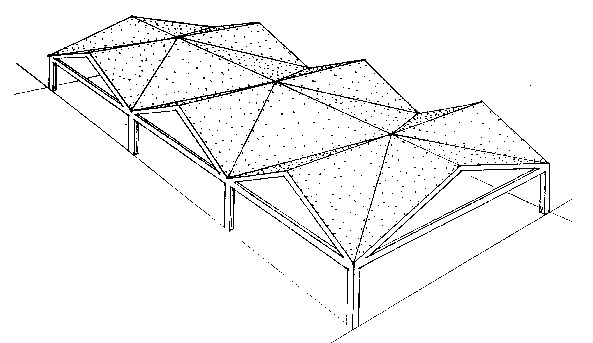
\includegraphics[width=.9\textwidth]{../figures/lipat}

\subsection{Struktur Cangkang}%
\label{ssub:Struktur Cangkang}


Struktur cangkang adalah sistem dengan pelat melengkung ke satu arah atau lebih yang tebalnya jauh lebih kecil daripada bentangnya. Gaya-gaya yang harus didukung dalam struktur cangkang disalurkan secara merata melalui permukaan bidang sebagai gaya-gaya membran yang diserap oleh elemen strukturnya. Gaya-gaya disalurkan sebagai gaya normal, dengan demikian tidak terdapat gaya lintang dan lentur. Resultan gaya yang tersebar diserap ke dalam struktur dengan gaya tangensial yang searah dengan kelengkungan bidang permukaannya.

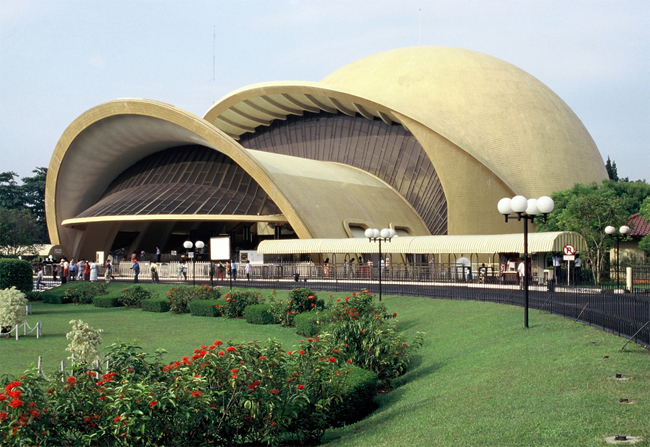
\includegraphics[width=.9\textwidth]{../figures/cangkang}


\subsection{Struktur membran}%
\label{sec:Struktur membran}


Struktur membran mempunyai prinsip yang sama dengan struktur cangkang, tetapi dengan bahan bidang permukaan yang sangat tipis. Kekakuan selaput tipis tersebut diperoleh dengan elemen tarik yang membentuk jala-jala yang saling membantu untuk menambah kapasitas menahan beban-beban lendutan.

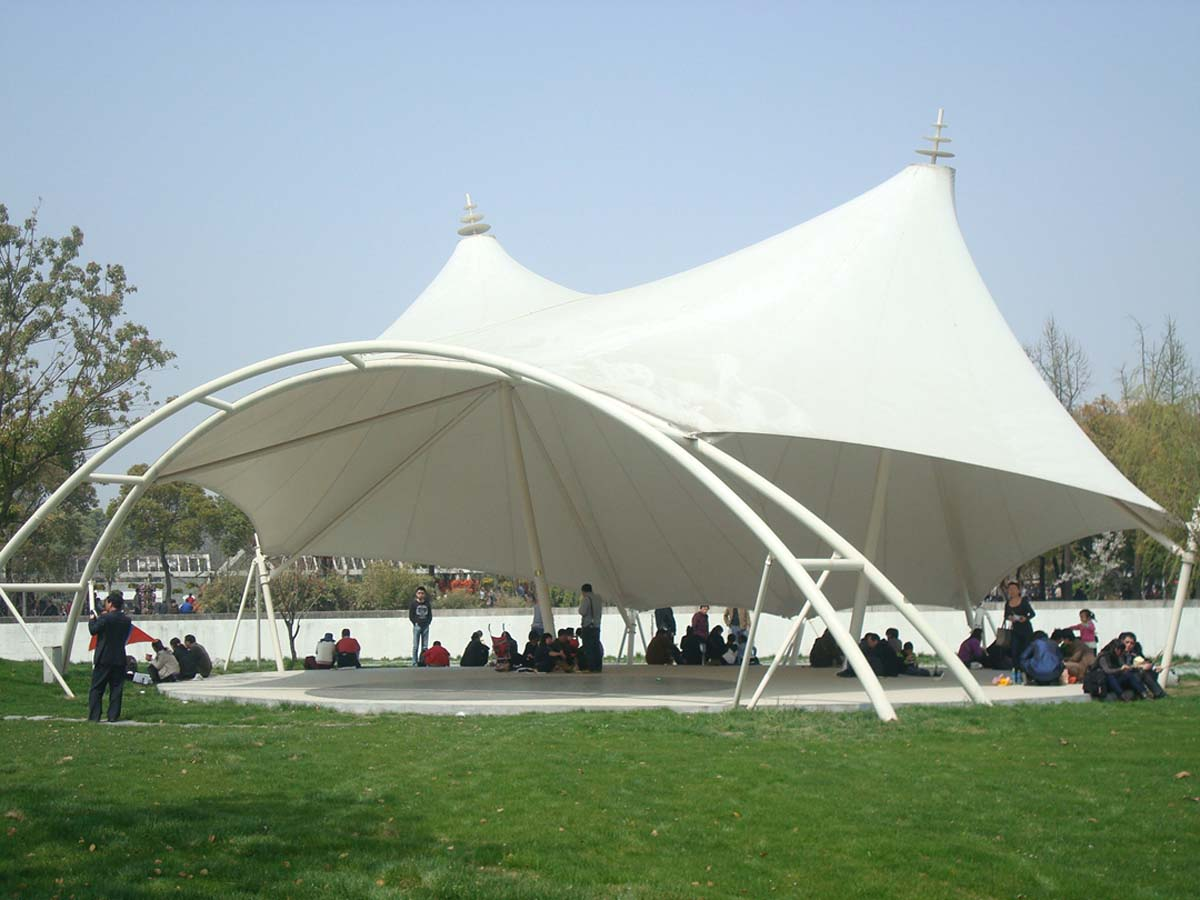
\includegraphics[width=.9\textwidth]{../figures/membran}

\subsection{Struktur Kabel dan Jaringan}%
\label{sec:Struktur Kabel dan Jaringan}


Struktur kabel dan jaringan dikembangkan dari kemampuan kabel menahan gaya tarik yang tinggi. Dengan menggunakan sistem tarik maka tidak diperlukan sistem penopang vertikal untuk elemen horisontalnya (lantai atau atap), sehingga daerah di bawah elemen horisontal (ruang) memiliki bentangan yang cukup besar. Bangunan dengan aplikasi sistem struktur in I akan sangat mendukung untuk bangunan bentang luas berbentang lebar, seperti dome, stadion, dll. Sistem yang dikembangkan pada struktur kabel antara lain :

\begin{itemize}
	\item Struktur atap tarik dengan kolom penunjang
	\item Struktur kabel tunggal
	\item Struktur kabel ganda
\end{itemize}

\subsubsection{Beban Vertikal (gravitasi)}%
\label{ssub:Beban Vertikal (gravitasi)}


\begin{itemize}
	\item Beban Mati (Dead Load).
	\item Beban Hidup (Live Load).
	\item Beban Air Hujan.
\end{itemize}

\subsubsection{Beban Horizontal}%
\label{ssub:Beban Horizontal}

\begin{itemize}\item Beban Gempa (Earthquake).
	\item Beban Angin (Wind Load).
	\item Tekanan Tanah dan Air Tanah.

\end{itemize}


\section{Perancangan Struktur Beton Bertulang}%
\label{sec:Perancangan Struktur Beton Bertulang}

\subsection{Perancangna Balok}%
\label{sub:Perancangna Balok}

Balok merupakan batang struktural untuk menahan gaya-gaya yang bekerja dalam arah tranversal terhadap sumbu yang mengakibatkan terjadinya lenturan. Menurut Wahyudi, L dan Rahim, S.A (1999) balok adalah elemen struktur yang didesain untuk menahan gaya-gaya yang bekerja secara transversal terhadap sumbunya sehingga mengakibatkan terjadinya lenturan. Dua hal utama yang dialami suatu balok adalah kondisi tekan dan tarik, yang antara lain karena adanya pengaruh lentur ataupun gaya lateral.
Untuk memperhitungkan kemampuan dan kapasitas dukung komponen balok struktur terlentur, sifat utama adalah kurang mampu menahan tarik akan menjadi dasar pertimbangan. Dengan cara memperkuat dengan penambahan tulangan baja pada daerah dimana tegangan tarik bekerja, akan diperoleh balok yang mampu menahan lentur.
Dalam perencanaan balok pada langkah awal ditentukan terlebih dahulu apakah balok tersebut berperilaku sebagai balok persegi atau balok T. Balok dianggap sebagai balok persegi jika seluruh daerah tekan terdapat pada daerah flens, sedangkan balok dianggap sebagai balok T jika seluruh daerah tekan terdapat dibawah daerah flens.









\bibliographystyle{apalike}
\bibliography{../filename.bib} % required for citecompletion, not work in mainfile
\end{document}

